\begin{figure}[!h]
  \begin{center}
    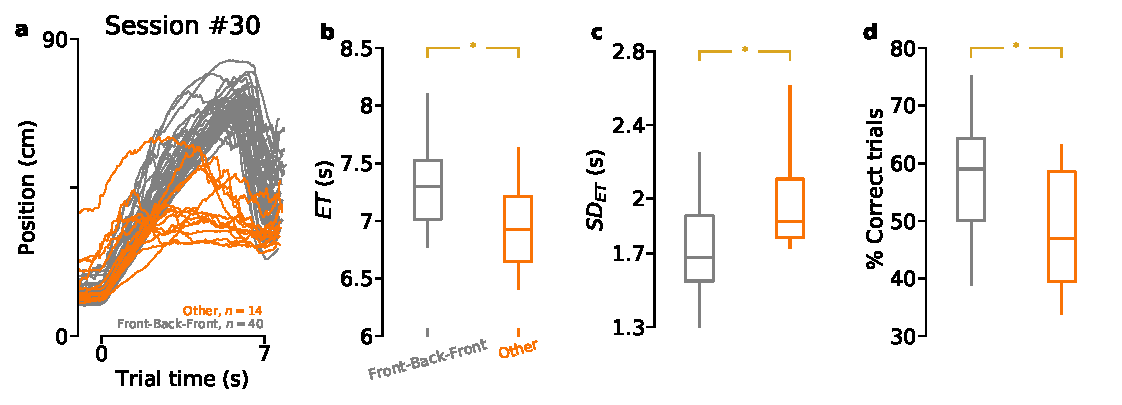
\includegraphics[width=\textwidth]{ch-appendicies/figures/BadCtrl.pdf}
    \caption[Different Control Trajectory Groups]
    {\textbf{Task proficiency according to the type of trajectory performed by animals.}
    \textbf{a)}
    Same as \autoref{fig:time:CtrlTrd}, panel~c,~right, but the animals were divided in two groups according to whether they performed the front-back-front trajectory (gray) or not (other, orange).
    \textbf{b)}
    Entrance times($ET$s).
    $p=0.0066$ (permutation test).
    \textbf{c)}
    $SD$ of $ET$.
    $p=0.03$ (permutation test).
    \textbf{d)}
    Percentage of correct trials.
    $p=0.01$ (permutation test).
    For panels~b,~c,~d, same color code as in panel~a.
    Data from sessions \#~$\geq20$ were averaged for each animal.
    }
    \label{fig:appendix:BadCtrl}
  \end{center}
\end{figure} 
